\section{Uppgift 9}\label{sec:uppg09}

\subsection{Instruktioner}
\begin{verbatim}
9. Skriv en klass Artikel som ska representera ett artikelslag på ett
   varulager. Information som ska finnas om varje artikelslag är:

   artikelnr (int), artikelnamn (String), lagerantal (int), pris
   (double)

   Denna information är alltså klassens instansvariabler, passande datatyp står
   inom parentes. I klassen ska även finnas en *klassvariabel* som håller
   räkning på hur många artikelslag det finns totalt, alltså som innehåller
   totala antalet skapade Artikel-objekt:

   totArtiklar (int)

   I klassen ska följande metoder ingå:

   * konstruktorn Artikel, som initierar samtliga instansvariabler samt
     uppdaterar klassvariabelns värde.
   * ändraNamn, metod som via parameter ändrar på artikelnamnet.
   * hamtaNamn, metod som returnerar artikelnamnet.
   * säljaArtikel, metod som minskar lagerantalet med parameterns värde.
   * fyllaLagret, metod som ökar lagerantalet med parameterns värde.
   * ändraPris, metod som ändrar priset till parameterns värde.
   * hamtaPris, metod som returnerar artikelns pris.
   * hamtaTotAntal, klassmetod som returnerar antalet artikelslag.
   * skrivInfo, metod av returtypen void som skriver ut alla data om en artikel.

   Skriv också ett testprogram, där du testar klassens alla metoder.
\end{verbatim}


\subsection{Källkod}
\javacode{src/main/Lab2Uppg09.java}
\caption{Lab2Uppg09.java}
\label{src:uppg09}

\javacode{src/main/Artikel.java}
\caption{Artikel.java}
\label{src:artikel}


\subsection{Skärmdump}
\begin{figure}[htbp]
    \centering
        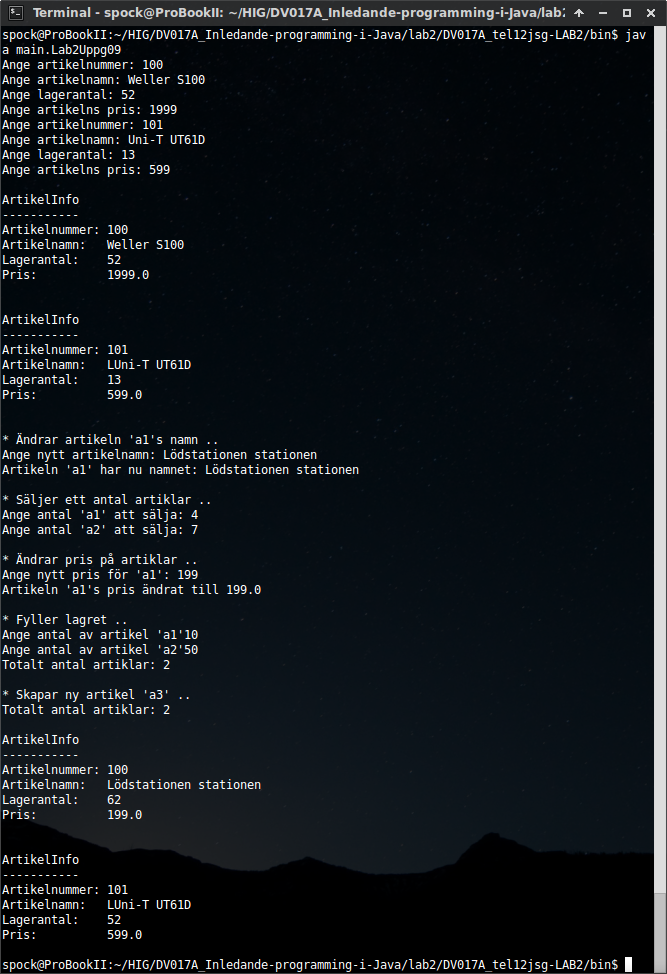
\includegraphics[width=\linewidth]{img/09.png}
    \caption{Körning av koden till Uppgift~\ref{sec:uppg09}}
    \label{fig:uppg09-screenshot}
\end{figure}

